% \documentclass[table]{beamer}
\documentclass[table,handout]{beamer}
\setbeameroption{show notes}
% \setbeameroption{hide notes}
% \setbeameroption{show only notes}
\usepackage{varwidth}

\newif\ifhide
\newif\ifpost
\newif\ifhideclicker

% \hidetrue
% \hideclickertrue
% \posttrue

\newcommand{\whiteout}[1]{\textcolor{white}{#1}}
% \newcommand{\whiteoutbox}[1]{\fcolorbox{white}{white}{\parbox{\dimexpr \linewidth-2\fboxsep-2\fboxrule}{\whiteout{#1}}}}
% \newcommand{\notebox}[1]{\fcolorbox{blue}{white}{\parbox{\dimexpr \linewidth-2\fboxsep-2\fboxrule}{#1}}}
\newcommand{\whiteoutbox}[1]{\fcolorbox{white}{white}{\parbox{\linewidth}{\whiteout{#1}}}}
\newcommand{\notebox}[1]{\fcolorbox{blue}{white}{\parbox{\linewidth}{#1}}}
\newcommand{\blankbox}[1]{\phantom{\varwidth{\linewidth}\whiteoutbox{#1}\endvarwidth}}
\newcommand{\blank}[1]{\phantom{\varwidth{\linewidth}#1\endvarwidth}}

\ifhide%
    \newcommand{\hmask}[1]{\blank{#1}}%
\else%
    \newcommand{\hmask}[1]{#1}%
\fi

\ifhide%
    \newcommand{\wout}[1]{\whiteout{#1}}%
\else%
    \newcommand{\wout}[1]{#1}%
\fi

\ifhide%
    \newcommand{\hignore}[1]{}%
\else%
    \newcommand{\hignore}[1]{#1}%
\fi

\ifpost%
    \newcommand{\nopost}[1]{}%
\else%
    \newcommand{\nopost}[1]{#1}%
\fi

\ifhideclicker%
    \newcommand{\clickerslide}[1]{\stepcounter{clickerQuestionCounter}%
        \begin{frame}[t]
            \textcolor{blue}{Q \arabic{clickerQuestionCounter}:}
        \end{frame}}
\else%
    \newcommand{\clickerslide}[1]{#1}%
\fi

\ifhide%
    \newcommand{\hidebox}[1]{\blank{#1}}%
\else%
    \newcommand{\hidebox}[1]{\notebox{#1}}%
\fi

\ifhide%
    \newcommand{\wbox}[1]{\whiteoutbox{#1}}%
\else%
    \newcommand{\wbox}[1]{\notebox{#1}}%
\fi

\ifhide%
    \newcommand{\nbox}[1]{\blankbox{#1}}%
\else%
    \newcommand{\nbox}[1]{\notebox{#1}}%
\fi

\ifhideclicker%
    \newcommand{\clickeranswer}[1]{#1}%
\else%
    \ifhide%
        \newcommand{\clickeranswer}[1]{#1}%
    \else%
        \newcommand{\clickeranswer}[1]{\textbf{\textcolor{blue}{#1}}}%
    \fi
\fi

\usepackage{beamerthemesplit}
% \usetheme{boxes}
\usetheme{Malmoe}
\usecolortheme{seahorse}
% \usecolortheme{seagull}
\usepackage{ifthen}
\usepackage{xspace}
\usepackage{multirow}
\usepackage{multicol}
\usepackage{booktabs}
\usepackage{xcolor}
\usepackage{wasysym}
\usepackage{comment}
\usepackage{hyperref}
\hypersetup{pdfborder={0 0 0}, colorlinks=true, urlcolor=blue, linkcolor=blue, citecolor=blue}
\usepackage{changepage}
\usepackage[compatibility=false]{caption}
\captionsetup[figure]{font=scriptsize, labelformat=empty, textformat=simple, justification=centering, skip=2pt}
\usepackage{tikz}
\usetikzlibrary{trees,calc,backgrounds}

\usepackage[bibstyle=joaks-slides,maxcitenames=3,mincitenames=1,backend=biber]{biblatex}

\newrobustcmd*{\shortfullcite}{\AtNextCite{\renewbibmacro{title}{}\renewbibmacro{in:}{}\renewbibmacro{number}{}}\fullcite}

\newrobustcmd*{\footlessfullcite}{\AtNextCite{\renewbibmacro{title}{}\renewbibmacro{in:}{}}\footfullcite}

% Make all footnotes smaller
% \renewcommand{\footnotesize}{\scriptsize}

\definecolor{myGray}{gray}{0.9}
\colorlet{rowred}{red!30!white}

\setbeamertemplate{blocks}[rounded][shadow=true]

\setbeamercolor{defaultcolor}{bg=structure!30!normal text.bg,fg=black}
\setbeamercolor{block body}{bg=structure!30!normal text.bg,fg=black}
\setbeamercolor{block title}{bg=structure!50!normal text.bg,fg=black}

\newenvironment<>{varblock}[2][\textwidth]{%
  \setlength{\textwidth}{#1}
  \begin{actionenv}#3%
    \def\insertblocktitle{#2}%
    \par%
    \usebeamertemplate{block begin}}
  {\par%
    \usebeamertemplate{block end}%
  \end{actionenv}}

\newenvironment{displaybox}[1][\textwidth]
{
    \centerline\bgroup\hfill
    \begin{beamerboxesrounded}[lower=defaultcolor,shadow=true,width=#1]{}
}
{
    \end{beamerboxesrounded}\hfill\egroup
}

\newenvironment{onlinebox}[1][4cm]
{
    \newbox\mybox
    \newdimen\myboxht
    \setbox\mybox\hbox\bgroup%
        \begin{beamerboxesrounded}[lower=defaultcolor,shadow=true,width=#1]{}
    \centering
}
{
    \end{beamerboxesrounded}\egroup
    \myboxht\ht\mybox
    \raisebox{-0.25\myboxht}{\usebox\mybox}\hspace{2pt}
}

\newenvironment{mydescription}{
    \begin{description}
        \setlength{\leftskip}{-1.5cm}}
    {\end{description}}

\newenvironment{myitemize}{
    \begin{itemize}
        \setlength{\leftskip}{-.3cm}}
    {\end{itemize}}

% footnote without a marker
\newcommand\barefootnote[1]{%
  \begingroup
  \renewcommand\thefootnote{}\footnote{#1}%
  \addtocounter{footnote}{-1}%
  \endgroup
}

% define formatting for footer
\newcommand{\myfootline}{%
    {\it
    \insertshorttitle
    \hspace*{\fill} 
    \insertshortauthor, \insertshortinstitute
    % \ifx\insertsubtitle\@empty\else, \insertshortsubtitle\fi
    \hspace*{\fill}
    \insertframenumber/\inserttotalframenumber}}

% set up footer
\setbeamertemplate{footline}{%
    \usebeamerfont{structure}
    \begin{beamercolorbox}[wd=\paperwidth,ht=2.25ex,dp=1ex]{frametitle}%
        % \Tiny\hspace*{4mm}\myfootline\hspace{4mm}
        \tiny\hspace*{4mm}\myfootline\hspace{4mm}
    \end{beamercolorbox}}

% remove navigation bar
\beamertemplatenavigationsymbolsempty

\makeatletter
    \newenvironment{noheadline}{
        \setbeamertemplate{headline}[default]
        \def\beamer@entrycode{\vspace*{-\headheight}}
    }{}
\makeatother

\newcounter{clickerQuestionCounter}
\ifhideclicker%
\newenvironment{clickerquestion}
{ \stepcounter{clickerQuestionCounter}
  \begin{enumerate}[Q \arabic{clickerQuestionCounter}:]\color{white} }
{ \end{enumerate} }
\else%
\newenvironment{clickerquestion}
{ \stepcounter{clickerQuestionCounter}
  \begin{enumerate}[Q \arabic{clickerQuestionCounter}:] }
{ \end{enumerate} }
\fi

\ifhideclicker%
\newenvironment{clickeroptions}
{ \begin{enumerate}[\begingroup\color{white} 1)\endgroup]\color{white} }
{ \end{enumerate} }
\else%
\newenvironment{clickeroptions}
{ \begin{enumerate}[\begingroup\color{red} 1)\endgroup] }
{ \end{enumerate} }
\fi


\tikzstyle{centered} = [align=center, text centered, font=\sffamily\bfseries]
\tikzstyle{skip} = [centered, inner sep=0pt, fill]
\tikzstyle{empty} = [centered, inner sep=0pt]
\tikzstyle{inode} = [centered, circle, minimum width=4pt, fill=black, inner sep=0pt]
\tikzstyle{tnode} = [centered, circle, inner sep=1pt]
\tikzset{
  % edge styles
  level distance=10mm,
  mate/.style={edge from parent/.style={draw,distance=3pt}},
  mleft/.style={grow=left, level distance=10mm, edge from parent path={(\tikzparentnode.west)--(\tikzchildnode.east)}},
  mright/.style={grow=right, level distance=10mm, edge from parent path={(\tikzparentnode.east)--(\tikzchildnode.west)}},
  % node styles
  male/.style={rectangle,minimum size=4mm,fill=gray!80},
  female/.style={circle,minimum size=4mm,fill=gray!80},
  amale/.style={male,fill=red},
  afemale/.style={female,fill=red},
}

\newcommand{\highlight}[1]{\textcolor{violet}{\textit{\textbf{#1}}}}
\newcommand{\super}[1]{\ensuremath{^{\textrm{\sffamily #1}}}}
\newcommand{\sub}[1]{\ensuremath{_{\textrm{\sffamily #1}}}}
\newcommand{\dC}{\ensuremath{^\circ{\textrm{C}}}}
\newcommand{\tb}{\hspace{2em}}
\providecommand{\e}[1]{\ensuremath{\times 10^{#1}}}
\newcommand{\myHangIndent}{\hangindent=5mm}

\newcommand{\spp}[1]{\textit{#1}}

\newcommand\mybullet{\leavevmode%
\usebeamertemplate{itemize item}\hspace{.5em}}

\makeatletter
\newcommand*{\rom}[1]{\expandafter\@slowromancap\romannumeral #1@}
\makeatother

\newcommand{\blankslide}{{\setbeamercolor{background canvas}{bg=black}
\setbeamercolor{whitetext}{fg=white}
\begin{frame}<handout:0>[plain]
\end{frame}}}

\newcommand{\whiteslide}{
\begin{frame}<handout:0>[plain]
\end{frame}}

\newcommand{\f}[1]{\ensuremath{F_{#1}}}
\newcommand{\x}[1]{X\ensuremath{^{#1}}}
\newcommand{\y}[1]{Y\ensuremath{^{#1}}}

% Population growth macros
\newcommand{\popsize}[1]{\ensuremath{N_{#1}}}
\newcommand{\popgrowthratediscrete}[1]{\ensuremath{\lambda_{#1}}}
\newcommand{\popgrowthrate}[1]{\ensuremath{r_{#1}}}
\newcommand{\ptime}{\ensuremath{t}\xspace}

\tikzset{hide on/.code={\only<#1>{\color{white}}}}
\tikzset{
    invisible/.style={opacity=0},
    visible on/.style={alt={#1{}{invisible}}},
    alt/.code args={<#1>#2#3}{%
        \alt<#1>{\pgfkeysalso{#2}}{\pgfkeysalso{#3}}
        % \pgfkeysalso doesn't change the path
    },
}

\bibliography{../bib/references}
\author[J.\ Oaks]{
    %Jamie R.\ Oaks\inst{1}
    Jamie R.\ Oaks
}
\institute[BIOL 180]{
    \inst{}%
        BIOL 180: Introductory Biology
}



\title[Innovations II: Animal diversification]{Innovations II: Animal
    diversification}
% \date{\today}
\date{May 7, 2015}


% \setbeamertemplate{section in toc}[sections numbered]
% \setbeamertemplate{subsection in toc}[subsections numbered]

\begin{document}

\begin{noheadline}
\maketitle
\end{noheadline}

\nopost{
\begin{noheadline}
\begin{frame}[c]
    \vspace{-6mm}
    \begin{center} 
        \includegraphics[height=1.2\textheight]{../images/seating-chart-2.pdf}
    \end{center}
\end{frame}
\end{noheadline}
}

\begin{noheadline}
\begin{frame}
\frametitle{Today's issues:}
\vspace{5mm}
% \tableofcontents[subsectionstyle=hide]
\tableofcontents
\end{frame}
\end{noheadline}

\section[What are animals?]{What are animals?}

\clickerslide{
\begin{frame}
    \begin{clickerquestion}
        \item The ``essence of plantness'' is to stay in one place, grow
            continuously throughout life, harvest diffuse resources (CO\sub{2},
            H\sub{2}0, nutrients in soil, sunlight), and synthesize complex
            molecules.  What is the equivalent ``essence of animalness?''

        \begin{clickeroptions}
            \item Multicellularity 
            \item Having a bilaterally symmetric, cephalized body.
            \item Having a coelom that creates a hydrostatic skeleton.
            \item \clickeranswer{Moving and harvesting concentrated packets of
                    resources.}
            \item Having tissues derived from ectoderm, endoderm, mesoderm.
        \end{clickeroptions}
    \end{clickerquestion}
\end{frame}
}

\clickerslide{
\begin{frame}
    \begin{clickerquestion}
        \item Most plants defend themselves against herbivores with toxins
            (they can't run away!). Extending this observation, which animal
            group is likely to have the most extensive suite of defense
            compounds?

        \begin{clickeroptions}
            \item Echinoderms (starfish, sea urchins, sea cucumbers)
            \item Gastropods (snails and slugs)
            \item \clickeranswer{Anthozoans (anemones and corals)}
            \item Insects
        \end{clickeroptions}
    \end{clickerquestion}

    \nbox{The logic here is that they don't move (as adults), and so have to
        have physical and/or chemical defenses (e.g., cnidocytes---ouch!!)}
\end{frame}
}

\begin{frame}
    \begin{adjustwidth}{-2em}{-1.5em}
        \vspace{-4mm}
        \begin{columns}[t]

            \column{0.47\linewidth}

            What are animals?

            \vspace{5mm}
            \begin{itemize}

                \item Moving and feeding machines

                \vspace{5mm}
                \item Most recent phylogeny

            \end{itemize}

            \column{0.52\linewidth}

                \vspace{-2mm}
                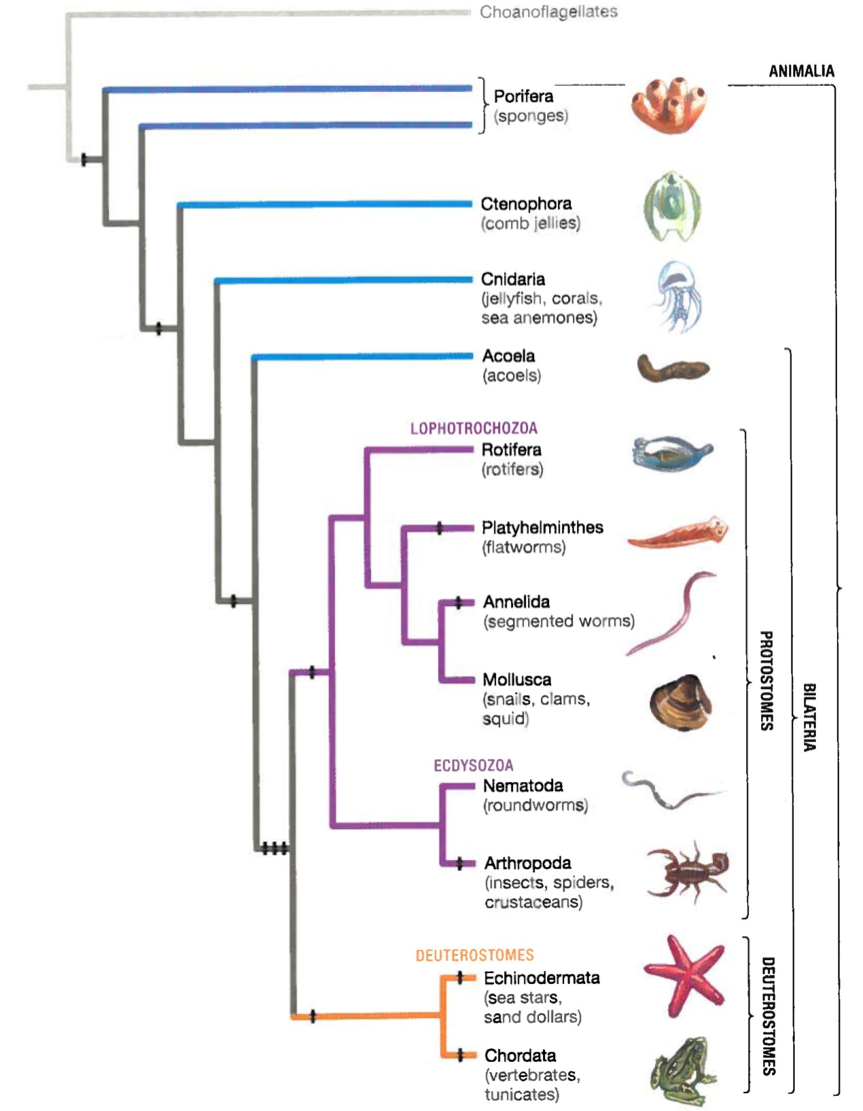
\includegraphics[height=\textheight]{animal-phylogeny-masked.png}

        \end{columns}
    \end{adjustwidth}

    \note[item]{Research (go dawgs) on ctenophores suggests simplicity in
        sponges is derived}
\end{frame}

\section[Evolution of animal body plan]{How did body plans change as animals
    diversified?}

\begin{frame}
    \begin{adjustwidth}{-2em}{-1.5em}
        How did body plans change as animals diversified?

        \begin{enumerate}

            \item Multicellularity and tissues

                \vspace{2mm}
                All animals are multicelluar

                \begin{itemize}

                    \item Cells bind to each other
                    \item Cells communicate
                    \item Division of labor (some cells function in feeding
                        vs.\ structure vs.\ reproduction)

                \end{itemize}

                Multicellularity evolved independently in fungi, plants, and
                several lineages of algae. Are the processes above the same or
                different?

                \nbox{Different---there should be similar functions (e.g.,
                    adhesion proteins, cell-to-cell signaling pathways,
                    hormones) performed by NON-homologous gene products.}

        \end{enumerate}
    \end{adjustwidth}
\end{frame}

\begin{frame}
    \begin{adjustwidth}{-2em}{-1.5em}
        \vspace{-4mm}
        \begin{columns}[t]

            \column{0.47\linewidth}

            Map the origin of \ldots

            \vspace{5mm}
            \begin{itemize}
                    \small

                \item Tissues (epithelium)

                    \nbox{\tiny Now accepted that sponges have epithelium, so
                        probably along the branch of the common ancestor of all
                        animals}

                \item Ectoderm

                    \nbox{\tiny Cnidaria and Ctenophora have endoderm +
                        ectoderm (no mesoderm), so along branch of ancestor of
                        all animals except sponges}

                \item Endoderm

                    \nbox{\tiny Cnidaria and Ctenophora have endoderm + ectoderm (no
                        mesoderm), so along branch of ancestor of all animals
                        except sponges}

                \item Mesoderm

                    \nbox{\tiny Bilaterians are triploblastic (endoderm +
                        ectoderm + mesoderm), so along branch of common
                        ancestor of all bilaterians.}

            \end{itemize}

            \column{0.52\linewidth}

                \vspace{-2mm}
                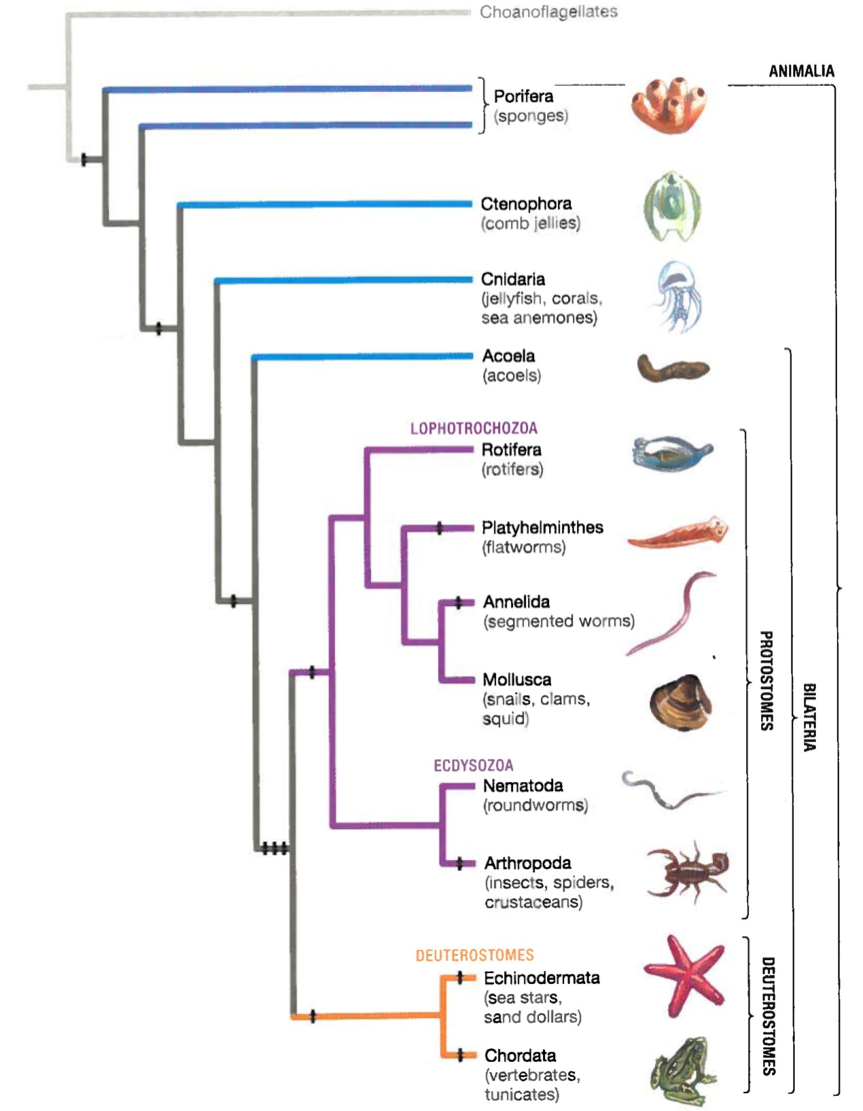
\includegraphics[height=\textheight]{animal-phylogeny-masked.png}

        \end{columns}
    \end{adjustwidth}

\end{frame}

\begin{frame}
    \begin{adjustwidth}{-2em}{-1.5em}
        \vspace{-4mm}
        \begin{columns}[t]

        \column{0.47\linewidth}
        \begin{enumerate}
            \addtocounter{enumi}{1}

            \item Body symmetry and cephalization
        \end{enumerate}

        {\small
        \uncover<2->{
        \vspace{2mm}
        Classically:

        \vspace{-2mm}
        \begin{itemize}

            \item Radial symmetry in diploblasts
            \item Bilateral symmetry in triploblasts
        \end{itemize}
        }

        \uncover<3->{
        But, we now know that some sponges are radially symmetric, and some
        cnidarian larvae are bilaterally symmetric.
        }

        \uncover<4->{
        \vspace{2mm}
        What does this suggest about the origin of symmetry types?

            \nbox{\tiny It's more complicated than we thought, and both
                radial and bilateral symmetry may have evolved much
                earlier than we thought}

        How could we explore this experimentally?

            \nbox{\tiny Look at the expression of genes involved during
                development of symmetry types (evo-devo); are they the same
                genes?}
        }
        }

        \column{0.52\linewidth}

            \vspace{-2mm}
            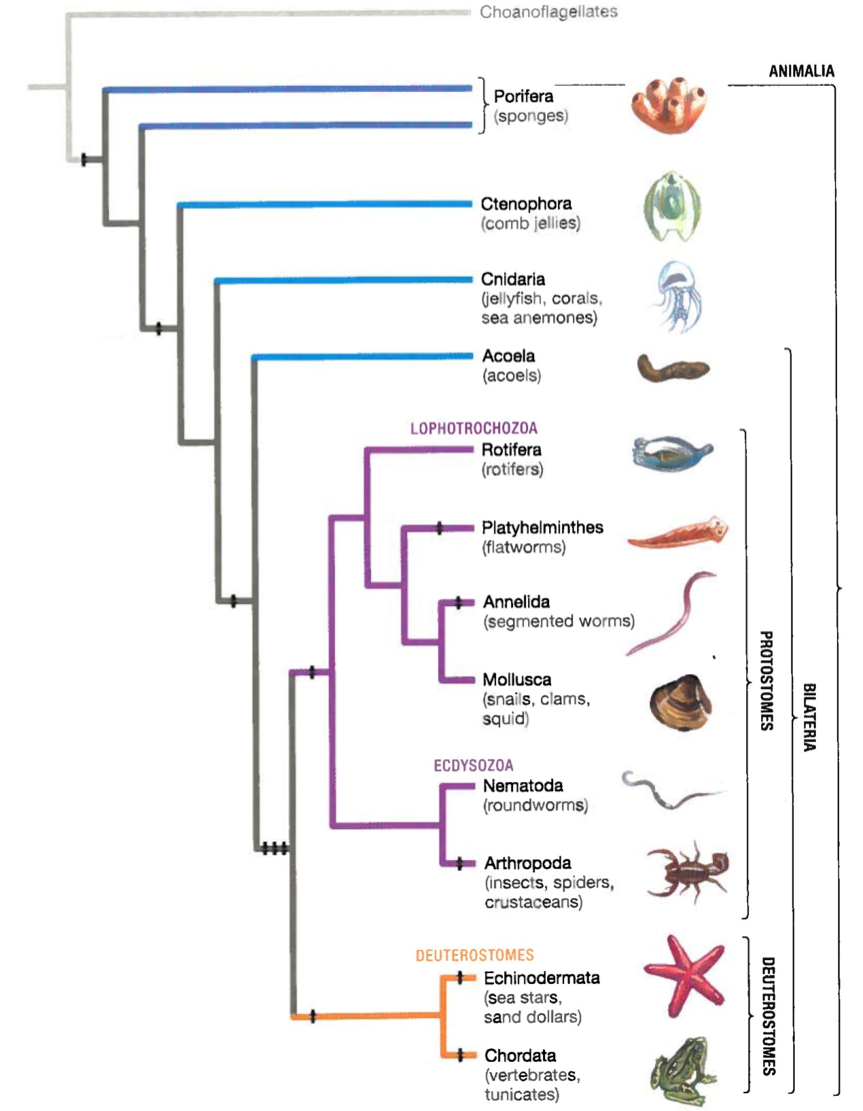
\includegraphics[height=\textheight]{animal-phylogeny-masked.png}

        \end{columns}
    \end{adjustwidth}
\end{frame}

\begin{frame}
    \begin{adjustwidth}{-2em}{-1.5em}
        \begin{columns}[t]
            \column{0.59\linewidth}

            Bilateral symmetry is (usually) associated with cephalization:
            \begin{enumerate}
                \item Centralized neurons
                \item Ganglia (brain) + sensory organs + mouth, all in head
                    region
            \end{enumerate}

            \uncover<2->{
            \vspace{2mm}
            Posterior region specialized for digestion, reproduction,
            locomotion.
            }

            \column{0.4\linewidth}

            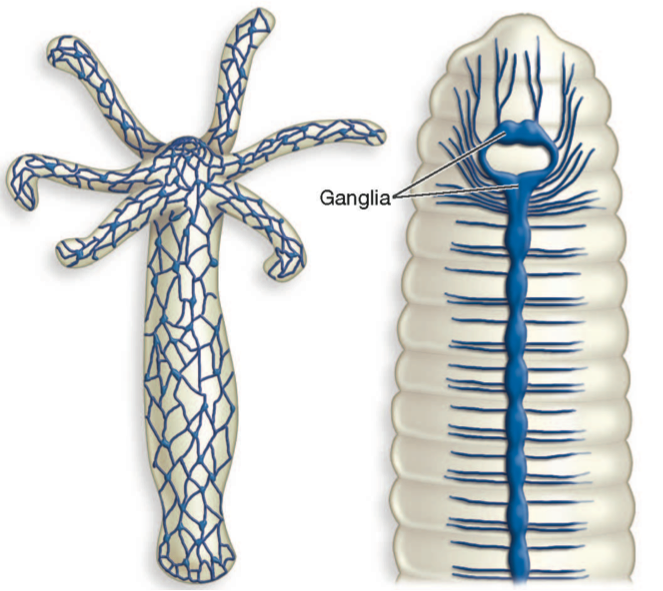
\includegraphics[width=\columnwidth]{bilateral-symmetry.png}
        \end{columns}

        \uncover<3->{
        What is the adaptive significance?

        \nbox{Consolidating nervous system makes for fast and efficient
            processing. Having all this processing power in the ``front''
            of the animal allows quick reaction to stimuli encountered
            while moving. Movement allows you to seek out pockets of
            resources.}
        }

    \end{adjustwidth}

    \note[item]{Label nerve net in hydra (cnidarian)---respond to stimuli in
        multiple directions.}
    \note[item]{Centralized nervous system in an earthworm---respond to stimuli
        in one direction.}
\end{frame}

\begin{frame}[t]
    \begin{adjustwidth}{-2em}{-1.5em}
        Echinoderms have radial symmetry in adults; larvae are bilaterally
        symmetric.

        \uncover<2->{
        \vspace{2mm}
        This is due to a ``reversion'' to radial symmetry

        \vspace{2mm}
        Is radial symmetry in echinoderms and cnidarians homologous?
        
        \nbox{No---homoplasy!}
        }

        \centering{
        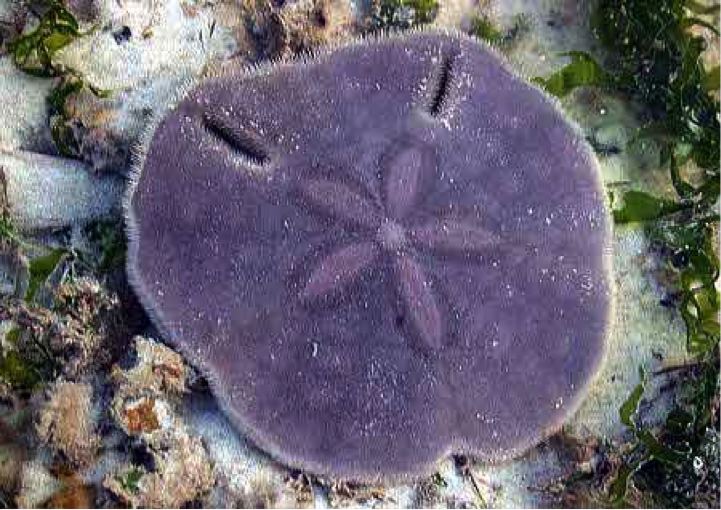
\includegraphics[height=0.5\textheight]{echinoderm-1.png}
        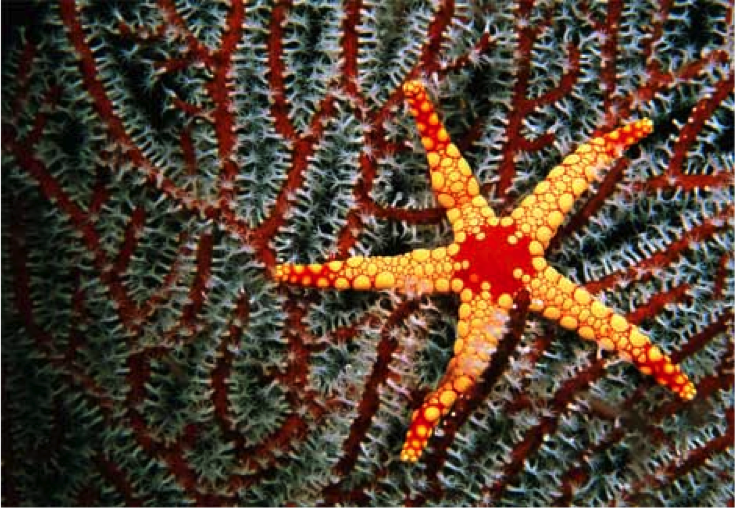
\includegraphics[height=0.5\textheight]{echinoderm-2.png}}

    \end{adjustwidth}

\end{frame}

\clickerslide{
\begin{frame}
    \begin{clickerquestion}
        \item Why don't biologists suggest that radial symmetry in echinoderms
            is homologous with radial symmetry in cnidarians (jellyfish,
            hydra, sea anemones)? 

        \begin{clickeroptions}
            \item Echinoderms appear much later in the fossil record. 
            \item \clickeranswer{All of the closet relatives of echinoderms are
                    NOT radially symmetric.}
            \item Echinoderms have a water vascular system as a synapomorphy. 
            \item Actually, it is!
        \end{clickeroptions}
    \end{clickerquestion}
\end{frame}
}

\begin{frame}[t]
    \begin{adjustwidth}{-2em}{-1.5em}
        \begin{enumerate}
            \addtocounter{enumi}{2}

            \item Evolution of a body cavity (coelom)

                \vspace{2mm}
                Tube-within-a-tube body design

                \vspace{2mm}
                Functions:

                \begin{itemize}

                    \item Hydrostatic skeleton important in movement
                    \item Space for internal organs, bathed in fluid
                \end{itemize}
        \end{enumerate}

    \end{adjustwidth}
    \note[item]{Draw the worm; draw the worm with legs}
\end{frame}

\clickerslide{
\begin{frame}
    \begin{clickerquestion}
        \item Most animals with legs have a reduced coelom or no coelom at all.
            Why? 

        \begin{clickeroptions}
            \item In these groups, the coelom is a vestigial trait. 
            \item Legs cannot develop if a coelom is present.
            \item \clickeranswer{The coelom's most important function has been
                    replaced, so there is no selection to maintain it.}
            \item They don't have a tube-within-a-tube body design.
        \end{clickeroptions}
    \end{clickerquestion}
\end{frame}
}

\clickerslide{
\begin{frame}
    \begin{clickerquestion}
        \item Why are groups that have vestigial coeloms---or that have lost
            coeloms entirely---considered ``coelomates?''

        \begin{clickeroptions}
            \item Because the coelom was such an important characteristic for
                fitness in early animal evolution.
            \item Just because a trait is vestigial doesn't mean that it has no
                function at all. 
            \item \clickeranswer{They evolved from ancestors that had a
                    coelom.}
            \item Evolutionary convergence has occurred many times. 
        \end{clickeroptions}
    \end{clickerquestion}
\end{frame}
}

\begin{frame}
    \begin{adjustwidth}{-2em}{-1.5em}
        \vspace{-4mm}
        \begin{columns}[t]

            \column{0.49\linewidth}

            \begin{enumerate}
                \addtocounter{enumi}{3}

                \item Developmental patterns

                \uncover<2->{
                \vspace{2mm}
                Classically:
                \begin{enumerate}
                    \item Protostome development

                    \begin{itemize}
                        \item Spiral cleavage
                        \item ``Mouth first'' gastrulation
                        \item Coelom from mesoderm blocks
                    \end{itemize}

                    \item Deuterostome development

                    \begin{itemize}
                        \item Radial cleavage
                        \item ``Mouth second'' gastrulation
                        \item Coelom from pinched-off mesoderm
                    \end{itemize}
                \end{enumerate}
                }
            \end{enumerate}

            \uncover<3->{
            {\small
            Recent work shows that arrow worms are sister to the protostomes.
            Arrow worms have radial cleavage and ``mouth-second'' gastrulation.
            }
            }

            \column{0.5\linewidth}

                \vspace{-2mm}
                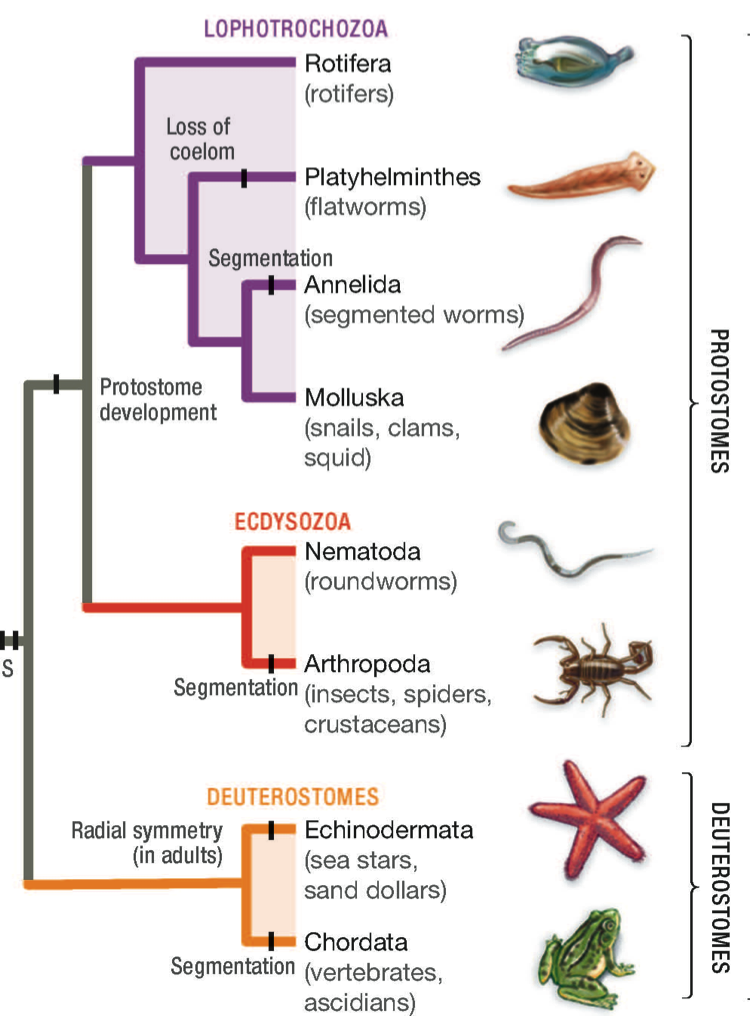
\includegraphics[width=\columnwidth]{animal-phylogeny-small.png}

        \end{columns}
    \end{adjustwidth}

\end{frame}

\clickerslide{
\begin{frame}
    \begin{clickerquestion}
        \item What is the most reasonable interpretation of the observation
            that arrow worms (chaetognaths) is the closest relative to
            protostomes?

        \begin{clickeroptions}
            \item At least some elements of protostome development are
                ancestral; deuterostome development is derived. 
            \item \clickeranswer{At least some elements of deuterostome
                    development are ancestral; protostome development is
                    derived.}
            \item Chaetognaths are weird (lots of homoplasy/loss).
        \end{clickeroptions}
    \end{clickerquestion}
\end{frame}
}

\begin{frame}[t]
    \begin{adjustwidth}{-2em}{-1.5em}

        \begin{enumerate}
            \addtocounter{enumi}{4}

            \item Segmentation 

                \vspace{2mm}
                Repeated structural units in a body: annelids (segmented worms),
                arthropods, vertebrates
        \end{enumerate}

        \centering{
        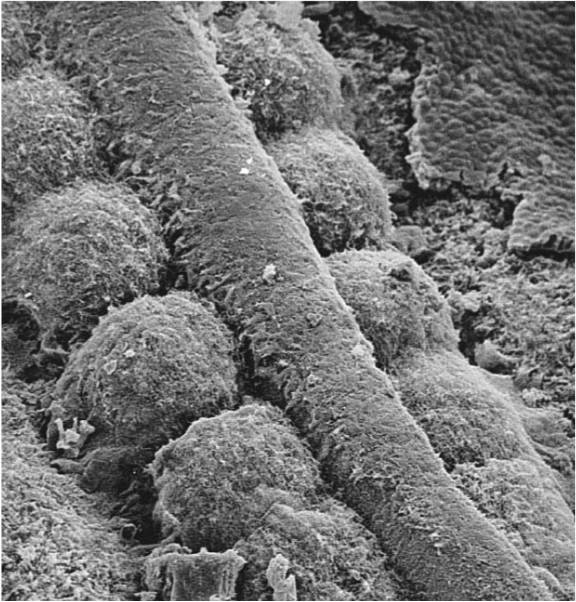
\includegraphics[height=0.55\textheight]{segmentation-1.png}
        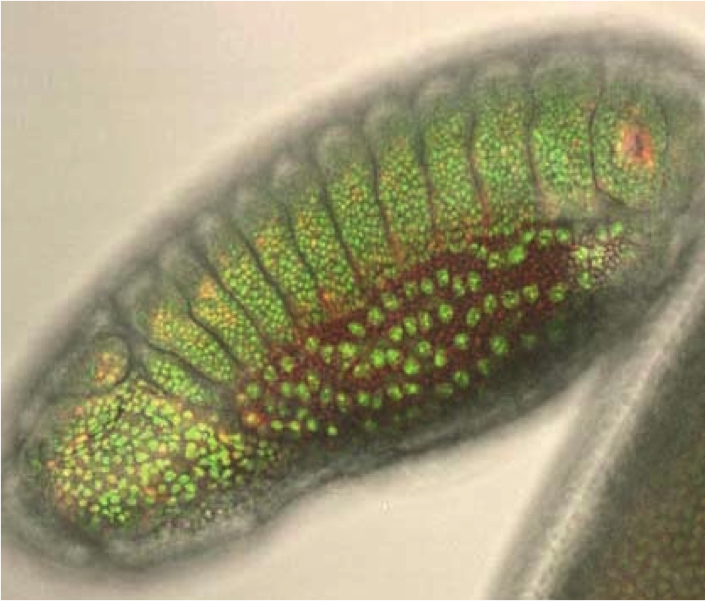
\includegraphics[height=0.55\textheight]{segmentation-2.png}}

    \end{adjustwidth}
\end{frame}

\clickerslide{
\begin{frame}
    \begin{clickerquestion}
        \item A recent paper showed that different genes are responsible for
            segmentation in annelids versus arthropods. Based on these data,
            which of the following is correct? 
 
        \begin{clickeroptions}
            \item Segmentation in annelids and arthropods is homologous
            \item The genes involved in vertebrate segmentation are homologous
                with annelid segmentation genes. 
            \item The genes involved in vertebrate segmentation are homologous
                with arthropod segmentation genes. 
            \item \clickeranswer{Segmentation in annelids and arthropods is an
                    example of homoplasy.}
        \end{clickeroptions}
    \end{clickerquestion}
\end{frame}
}

\begin{frame}[t]
    \begin{adjustwidth}{-2em}{-1.5em}

        \vspace{-4mm}
        \begin{columns}[t]

            \column{0.47\linewidth}

        \begin{enumerate}
            \addtocounter{enumi}{5}

            \item Growth patterns

                \begin{itemize}
                    \item Molting vs.\ continuous growth

                        \vspace{5mm}
                    \item Metamorphosis

                        \nbox{Larval state has distinct body, habitat, and
                            feeding (often dispersal as larva). Many insects,
                            crustaceans, mollusks, annelids.}
                \end{itemize}

        \end{enumerate}

            \column{0.52\linewidth}

        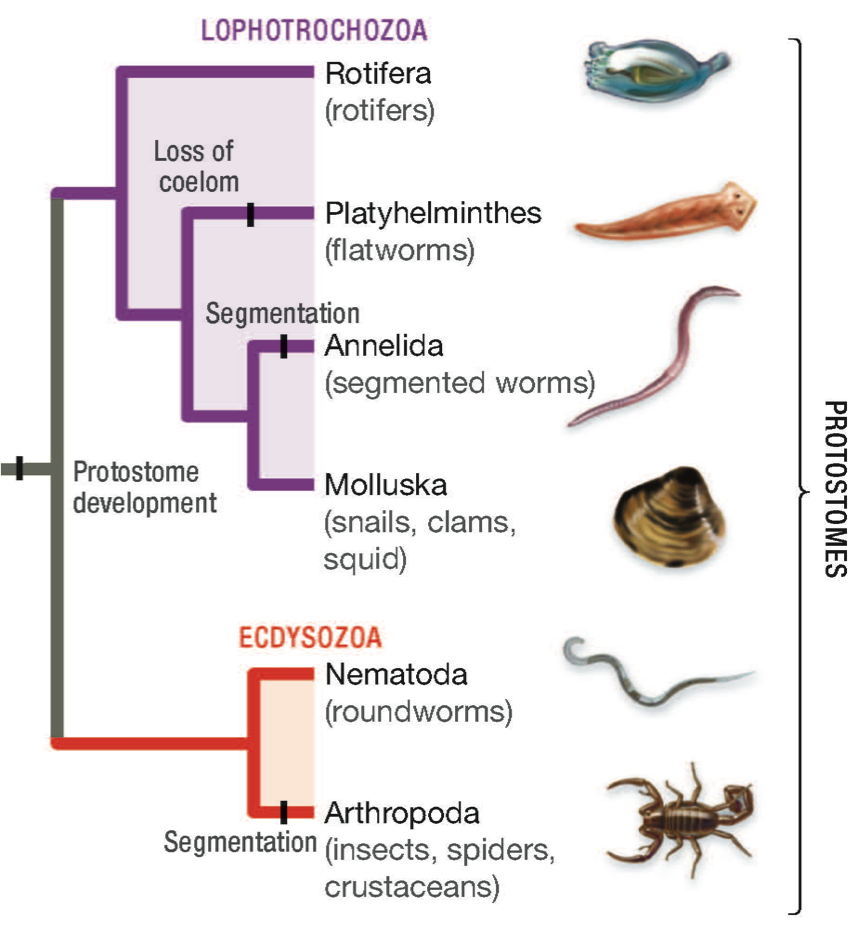
\includegraphics[width=\columnwidth]{animal-phylogeny-zoom.png}

        \end{columns}
    \end{adjustwidth}
\end{frame}

\begin{frame}
    \begin{adjustwidth}{-2em}{-1.5em}
        \vspace{-4mm}
        \begin{columns}[t]

            \column{0.47\linewidth}

            Questions:

            \begin{itemize}

                \item Are annelids more derived than sponges?

                    \nbox{No---the groups are derived from the same common
                        ancestor. BUT, it is correct to say that sponges have
                        an ancestral form of a trait and annelids have a
                        derived form of a trait.}

                \item Is loss of the coelom in mollusks, echinoderms, and
                    chordates homologous?

                    \nbox{No---It's homoplastic. It happened independently, and
                        for different reasons (different traits took over the
                        coelom's functions).}

            \end{itemize}

            \column{0.52\linewidth}

                \vspace{-1.5mm}
                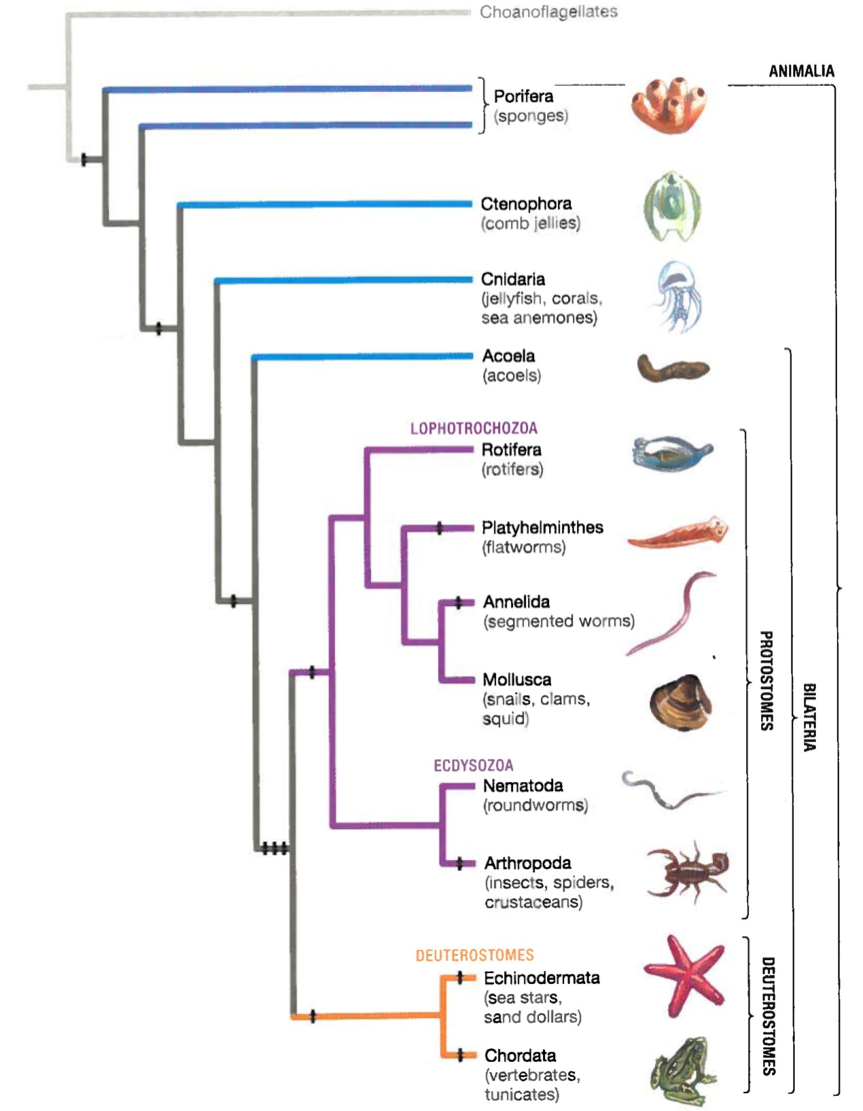
\includegraphics[height=\textheight]{animal-phylogeny-masked.png}

        \end{columns}
    \end{adjustwidth}
\end{frame}

\end{document}

\clickerslide{
\begin{frame}
    \begin{clickerquestion}
        \item 
        \begin{clickeroptions}
            \item 
            \item 
            \item 
            \item 
        \end{clickeroptions}
    \end{clickerquestion}
\end{frame}
}

\clickerpost{
{
\usebackgroundtemplate{\includegraphics[page=17,width=\paperwidth]{./24-Radiation-extinction.pdf}}
\begin{frame}[t,plain]
    \begin{adjustwidth}{-2em}{-1.5em}
        \cmask{Answer: 3}
    \end{adjustwidth}
\end{frame}
}
}

